%\documentclass[pra,showpacs,showkeys,amsfonts,amsmath,twocolumn]{revtex4}
\documentclass[amsmath,table,sans,amsfonts, handout]{beamer}
%\documentclass[pra,showpacs,showkeys,amsfonts]{revtex4}
\usepackage[T1]{fontenc}
%%\usepackage{beamerthemeshadow}
%%\usepackage[headheight=1pt,footheight=10pt]{beamerthemeboxes}
%%\addfootboxtemplate{\color{structure!80}}{\color{white}\tiny \hfill Karl Svozil (TU Vienna)\hfill}
%%\addfootboxtemplate{\color{structure!65}}{\color{white}\tiny \hfill mur.sat \hfill}
%%\addfootboxtemplate{\color{structure!50}}{\color{white}\tiny \hfill Graz, 2010-12-11\hfill}
%\usepackage[dark]{beamerthemesidebar}
%\usepackage[headheight=24pt,footheight=12pt]{beamerthemesplit}
%\usepackage{beamerthemesplit}
%\usepackage[bar]{beamerthemetree}
\usepackage{graphicx}
\usepackage{pgf}
%\usepackage{eepic}
%\usepackage[usenames]{color}
%\newcommand{\Red}{\color{Red}}  %(VERY-Approx.PANTONE-RED)
%\newcommand{\Green}{\color{Green}}  %(VERY-Approx.PANTONE-GREEN)

%\RequirePackage[german]{babel}
%\selectlanguage{german}
%\RequirePackage[isolatin]{inputenc}

%\pgfdeclareimage[height=0.5cm]{logo}{tu-logo}
%\logo{\pgfuseimage{logo}}
\beamertemplatetriangleitem
%\beamertemplateballitem

\beamerboxesdeclarecolorscheme{alert}{red}{red!15!averagebackgroundcolor}
%\begin{beamerboxesrounded}[scheme=alert,shadow=true]{}
%\end{beamerboxesrounded}

%\beamersetaveragebackground{yellow!10}

%\beamertemplatecircleminiframe

\newtheorem{question}{Question}
\newtheorem{conjecture}[question]{Principle}
\newtheorem{challenge}[question]{Challenge}
\usepackage{tikz}
\newcommand{\bra}[1]{\left< #1 \right|}
\newcommand{\ket}[1]{\left| #1 \right>}

\newcommand{\iprod}[2]{\langle #1 | #2 \rangle}
\newcommand{\mprod}[3]{\langle #1 | #2 | #3 \rangle}
\newcommand{\oprod}[2]{| #1 \rangle\langle #2 |}

\newcommand{\proj}[3]{\begin{smallmatrix} #1 & #2 & #3 \end{smallmatrix}}
\newcommand{\projbf}[3]{\begin{smallmatrix} \mathbf{#1} & \mathbf{#2} & \mathbf{#3} \end{smallmatrix}}

\sloppy
\parskip .7em %vskip between paragraphs

\newcommand{\seq}[1]{\mathbf{#1}}
\newcommand{\floor}[1]{\left\lfloor #1 \right\rfloor}
\newcommand{\ceil}[1]{\left\lceil #1 \right\rceil}
\newcommand{\m}[1]{\widetilde{#1}}
\newcommand{\p}[1]{\scriptsize\textcolor{black}{$[#1]$}}

\begin{document}

\title{\bf \textcolor{blue}{The present situation in quantum mechanics and the ontological single pure state conjecture}}
\subtitle{\textcolor{orange!60}{\small http://tph.tuwien.ac.at/$\sim$svozil/publ/2012-cagliari-IQSA12-pres.pdf
\\
http://arxiv.org/abs/1206.6024  (v2 from tomorrow on)
}}
\author{Karl Svozil}
\institute{University of Technology Vienna, Austria\\
vistiting\\
The University of Cagliari, Italy \\
The University of Auckland, New Zealand \\
%Wiedner Hauptstra\ss e 8-10/136, A-1040 Vienna, Austria\\
svozil@tuwien.ac.at
%{\tiny Disclaimer: Die hier vertretenen Meinungen des Autors verstehen sich als Diskussionsbeitr�ge und decken sich nicht notwendigerweise mit den Positionen der Technischen Universit�t Wien oder deren Vertreter.}
}
\date{Cagliari, July 23th, 2012}
\maketitle


%\frame{
%\frametitle{Contents}
%\tableofcontents
%}


\frame{
\frametitle{Advertisement for a paper by Abbot, Calude, Conder \& K.S., eprint arXiv:1207.2029}
\begin{Corollary}
\label{cor:twonotvaluedefinite}
	Let $a$ and $b$ be two observables that project onto one-dimensional subspaces $A$ and $B$ of the Hilbert space $\mathbb{C}^3$.
	Suppose there are unit vectors $\ket{a}\in A$ and $\ket{b}\in B$ such that $\sqrt{\frac{5}{14}} \le |\iprod{a}{b}| \le \frac{3}{\sqrt{14}}\raisebox{.8mm}{.}$
	Then there exists a set of projection observables $\mathcal{O}$ containing $a$ and $b$, and a set of contexts $\mathcal{C}$ over $\mathcal{O}$, such that there is no admissible assignment function under which $\mathcal{O}$ is non-contextual, $a$ has the value 1 and $b$ is value definite.
\end{Corollary}
}

\frame{
\frametitle{Advertisement for a paper by Abbot, Calude, Conder \& K.S., eprint arXiv:1207.2029, Greechie diagram of proof}
\begin{center}
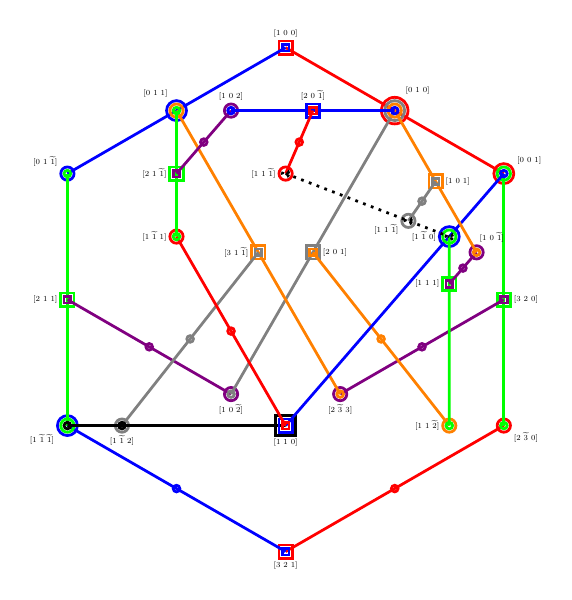
\begin{tikzpicture}   [scale=0.4, transform shape]
\tikzstyle{every path}=[line width=1pt]
\tikzstyle{every node}=[draw,line width=1pt,inner sep=2]
\tikzstyle{Hidden}=[draw opacity=0]

\tikzstyle{y1}=[rectangle,minimum size=6]
\tikzstyle{y2}=[rectangle,minimum size=12]
\tikzstyle{y3}=[rectangle,minimum size=18]
\tikzstyle{y4}=[rectangle,minimum size=24]

\tikzstyle{n1}=[circle,minimum size=6]
\tikzstyle{n2}=[circle,minimum size=12]
\tikzstyle{n3}=[circle,minimum size=18]
\tikzstyle{n4}=[circle,minimum size=24]

\tikzstyle{l1}=[draw=none,rectangle,minimum size=6]
\tikzstyle{l2}=[draw=none,rectangle,minimum size=12]
\tikzstyle{l3}=[draw=none,rectangle,minimum size=18]
\tikzstyle{l4}=[draw=none,rectangle,minimum size=24]

\draw[red] (90:8) -- (30:8)
	coordinate[y2,at start] (1 0 0)
	coordinate[n4,midway] (0 1 0)
	coordinate[n3,at end] (0 0 1);

\draw[blue] (1 0 0.center) -- (150:8)
	coordinate[y1,at start] (1 0 0)
	coordinate[n3,midway] (0 1 1)
	coordinate[n2,at end] (0 1 -1);

\draw[red] (270:8) -- (330:8)
	coordinate[y2,at start] (3 2 1)
	coordinate[n1,midway] (3 2 -13)
	coordinate[n2,at end] (2 -3 0);

\draw[blue] (3 2 1.center) -- (210:8)
	coordinate[y1,at start] (3 2 1)
	coordinate[n1,midway] (1 -4 5)
	coordinate[n3,at end] (1 -1 -1);

\draw[green] (1 -1 -1.center) -- (0 1 -1.center)
	coordinate[n2,at start] (1 -1 -1)
	coordinate[y2,midway] (2 1 1)
	coordinate[n1,at end] (0 1 -1);

\draw[green] (2 -3 0.center) -- (0 0 1.center)
	coordinate[n1,at start] (2 -3 0)
	coordinate[y2,midway] (3 2 0)
	coordinate[n2,at end] (0 0 1);

\draw[Hidden] (2 1 1.center) -- (3 2 -13.center)
	coordinate[midway] (1 0 -2);

\draw[Hidden] (3 2 0.center) -- (1 -4 5.center)
	coordinate[midway] (2 -3 3);

\draw[violet] (2 1 1.center) -- (1 0 -2.center)
	coordinate[y1,at start] (2 1 1)
	coordinate[n1,midway] (2 -5 1)
	coordinate[n2,at end] (1 0 -2);

\draw[violet] (3 2 0.center) -- (2 -3 3.center)
	coordinate[y1,at start] (3 2 0)
	coordinate[n1,midway] (6 -9 -13)
	coordinate[n2,at end] (2 -3 3);

\draw[gray] (0 1 0.center) -- (1 0 -2.center)
	coordinate[n3,at start] (0 1 0)
	coordinate[y2,midway] (2 0 1)
	coordinate[n1,at end] (1 0 -2);

\draw[orange] (0 1 1.center) -- (2 -3 3.center)
	coordinate[n2,at start] (0 1 1)
	coordinate[y2,midway] (3 1 -1)
	coordinate[n1,at end] (2 -3 3);

\draw[Hidden] (1 -1 -1.center) -- (2 -3 0.center)
	coordinate[very near start] (1 -1 2)
	coordinate[midway] (1 1 0)
	coordinate[very near end] (1 1 -2);

\draw[orange] (2 0 1.center) -- (1 1 -2.center)
	coordinate[y1,at start] (2 0 1)
	coordinate[n1,midway] (1 -5 -2)
	coordinate[n2,at end] (1 1 -2);

\draw[gray] (3 1 -1.center) -- (1 -1 2.center)
	coordinate[y1,at start] (3 1 -1)
	coordinate[n1,midway] (1 -7 -4)
	coordinate[n2,at end] (1 -1 2);

\draw[black] (1 -1 -1.center) -- (1 1 0.center)
	coordinate[n1,at start] (1 -1 -1)
	coordinate[n1,near start] (1 -1 2)
	coordinate[y3,at end] (1 1 0);

\draw[blue] (1 1 0.center) -- (0 0 1.center)
	coordinate[y2,at start] (1 1 0)
	coordinate[n3,near end] (1 -1 0)
	coordinate[n1,at end] (0 0 1);

\draw[Hidden] (0 1 -1.center) -- (2 -3 0.center)
	coordinate[near start] (1 -1 1);

\draw[red] (1 1 0.center) -- (1 -1 1.center)
	coordinate[y1,at start] (1 1 0)
	coordinate[n1,midway] (1 -1 -2)
	coordinate[n2,at end] (1 -1 1);

\draw[green] (1 -1 0.center) -- (1 1 -2.center)
	coordinate[n2,at start] (1 -1 0)
	coordinate[y2,near start] (1 1 1)
	coordinate[n1,at end] (1 1 -2);

\draw[green] (1 -1 1.center) -- (0 1 1.center)
	coordinate[n1,at start] (1 -1 1)
	coordinate[y2,midway] (2 1 -1)
	coordinate[n1,at end] (0 1 1);

\draw[Hidden] (0 1 0.center) -- (3 2 0.center)
	coordinate[near end] (1 0 -1);

\draw[Hidden] (0 1 0.center) -- (0 1 1.center)
	coordinate[near end] (1 0 2);

\draw[violet] (1 1 1.center) -- (1 0 -1.center)
	coordinate[y1,at start] (1 1 1)
	coordinate[n1,midway] (1 -2 1)
	coordinate[n2,at end] (1 0 -1);

\draw[violet] (2 1 -1.center) -- (1 0 2.center)
	coordinate[y1,at start] (2 1 -1)
	coordinate[n1,midway] (2 -5 -1)
	coordinate[n2,at end] (1 0 2);

\draw[orange] (1 0 -1.center) -- (0 1 0.center)
	coordinate[n1,at start] (1 0 -1)
	coordinate[y2,midway] (1 0 1)
	coordinate[n2,at end] (0 1 0);

\draw[blue] (1 0 2.center) -- (0 1 0.center)
	coordinate[n1,at start] (1 0 2)
	coordinate[y2,midway] (2 0 -1)
	coordinate[n1,at end] (0 1 0);

\draw[Hidden] (1 0 0.center) -- (3 2 1.center)
	coordinate[near start] (1 1 2);

\draw[Hidden] (1 1 2.center) -- (1 -1 0.center)
	coordinate[near end] (1 1 -1);

\draw[gray] (1 0 1.center) -- (1 1 -1.center)
	coordinate[y1,at start] (1 0 1)
	coordinate[n1,midway] (1 -2 -1)
	coordinate[n2,at end] (1 1 -1);

\draw[red] (2 0 -1.center) -- (1 1 2.center)
	coordinate[y1,at start] (2 0 -1)
	coordinate[n1,midway] (1 -5 2)
	coordinate[n2,at end] (1 1 2);

\draw[dotted] (1 1 2.center) -- (1 -1 0.center)
	coordinate[n1,at start] (1 1 2)
	coordinate[n1,near end] (1 1 -1)
	coordinate[n1,at end] (1 -1 0);

\coordinate[l2,label=90:\p{1~0~0}] (1 0 0) at (1 0 0.center);
\coordinate[l4,label=60:\p{0~1~0}] (0 1 0) at (0 1 0.center);
\coordinate[l3,label=30:\p{0~0~1}] (0 0 1) at (0 0 1.center);

\coordinate[l3,label=120:\p{0~1~1}] (0 1 1) at (0 1 1.center);
\coordinate[l2,label=150:\p{0~1~\m1}] (0 1 -1) at (0 1 -1.center);

\coordinate[l2,label=270:\p{3~2~1}] (3 2 1) at (3 2 1.center);
\coordinate[l2,label=330:\p{2~\m3~0}] (2 -3 0) at (2 -3 0.center);
\coordinate[l3,label=210:\p{1~\m1~\m1}] (1 -1 -1) at (1 -1 -1.center);

\coordinate[l2,label=180:\p{2~1~1}] (2 1 1) at (2 1 1.center);
\coordinate[l2,label=0:\p{3~2~0}] (3 2 0) at (3 2 0.center);

\coordinate[l2,label=270:\p{1~0~\m2}] (1 0 -2) at (1 0 -2.center);
\coordinate[l2,label=270:\p{2~\m3~3}] (2 -3 3) at (2 -3 3.center);

\coordinate[l2,label=0:\p{2~0~1}] (2 0 1) at (2 0 1.center);
\coordinate[l2,label=180:\p{3~1~\m1}] (3 1 -1) at (3 1 -1.center);

\coordinate[l2,label=180:\p{1~1~\m2}] (1 1 -2) at (1 1 -2.center);
\coordinate[l2,label=270:\p{1~\m1~2}] (1 -1 2) at (1 -1 2.center);

\coordinate[l3,label=270:\p{1~1~0}] (1 1 0) at (1 1 0.center);

\coordinate[l3,label=180:\p{1~\m1~0}] (1 -1 0) at (1 -1 0.center);
\coordinate[l2,label=180:\p{1~\m1~1}] (1 -1 1) at (1 -1 1.center);

\coordinate[l2,label=180:\p{1~1~1}] (1 1 1) at (1 1 1.center);
\coordinate[l2,label=180:\p{2~1~\m1}] (2 1 -1) at (2 1 -1.center);

\coordinate[l2,label=87.5:\p{1~0~\m1}] (1 0 -1) at (1 0 -1.center);
\coordinate[l2,label=90:\p{1~0~2}] (1 0 2) at (1 0 2.center);

\coordinate[l2,label=0:\p{1~0~1}] (1 0 1) at (1 0 1.center);
\coordinate[l2,label=90:\p{2~0~\m1}] (2 0 -1) at (2 0 -1.center);

\coordinate[l2,label=185:\p{1~1~\m1}] (1 1 -1) at (1 1 -1.center);
\coordinate[l2,label=180:\p{1~1~\m1}] (1 1 2) at (1 1 2.center);
\end{tikzpicture}
\end{center}

}


\section{Persistent issues}

\frame{
\frametitle{Persistent issues}
Quite rightly quantum mechanics has been lauded as one of the most successful physical theories ever developed by human thought.
Yet at the same time non-negligible areas of its formalism, let alone its interpretation, remain conceptually fuzzy and unclear.
In this respect, the situation is not too different today than it has been almost a century ago,
when Schr\"odinger published his famous series of articles
on the conceptual difficulties troubling the formal framework which he had helped to create.
}

\section{Do measurements exist?}
\frame{
\frametitle{Do measurements exist?}

The late Bell sarcastically observed that, just as Dirac, most quantum physicists appear to be
``why bother?'ers''  who might just as well neglect the
measurement problem by considering it solved {\color{blue} ``for all practical purposes'' (FAPP)}.
Yet, the associated issues are much more pressing now then ever,
as technologies based on quantum concepts of measurement
have been applied for experiments,
as well as deployed for cryptanalysis and industry.
In particular, at stake is the nature of randomness emerging from such devices.

}


\subsection{Quantum jellification}

\frame{
\frametitle{Quantum jellification}

Already around 1935, Schr\"odinger considered the {\em coherent superposition}
$\vert 0 \rangle + \vert 1 \rangle$ of classically distinct, mutually exclusive and operationally separable states
$\vert 0 \rangle$
and
$\vert 1 \rangle$,
which is a direct consequence of the linear vector space formalism,
as a serious issue.
He expressed this metaphorically by a cat in a {\em coherent superposition}
``between being dead and alive'' $\vert D \rangle + \vert A \rangle$; the latter state being somehow
``induced'' by the coherent superposition of a single two-state quantum by some unspecified but supposedly hypothetical quantum evolution
$$
\vert 0 \rangle + \vert 1 \rangle \mapsto \vert D \rangle + \vert A \rangle
$$
``blowing up'' the microscopic coherence into the classical domain.
}
\frame{
\frametitle{Quantum jellification cntd.}

In 1952, Schr\"odinger maintained  that, quite generally,
without measurement, quantum theorists should be troubled that, due to coherent superposition
resulting in the co-existence of classically mutually exclusive alternatives,
their  {\color{blue} ``surroundings rapidly turning into a quagmire, a sort of a featureless jelly or plasma,
all contours becoming blurred, we ourselves probably becoming jelly fish.''}

}

\subsection{Everett and Wigner's observation of a subjective observer-object cut}

\frame{
\frametitle{Everett and Wigner's observation of a subjective observer-object cut}

Around that time,
Everett  and  Wigner
observed that,
if a unitary (bijective, one-to-one, reversible, Laplacian-type deterministic) quantum evolution were universally valid,
then any distinction or cut between the observer and the measurement apparatus necessarily remains not absolute or ontic,
but epistemic, subjective and conventional.

Because, suppose that one has defined a cut or difference between an observed quantum and a ``quasi-classical'' measurement device,
one could, at least in principle and if the unitary quantum evolution is universally valid,
``draw a larger perimeter.'' This `` `enlargement'' could encompass the entire previous combination,
{\em including} the quantum, the cut, and the measurement device.
If the quantum laws are universally valid, such a quantized system should also undergo
a unitary quantum evolution.
Hence, any ``irreversibility'' decays into ``thin air.''


}

\subsection{Formal and empirical aspects of (ir-)reversibility}

\frame{
\frametitle{`Emergence' of many-to-one from one-to-one functions?}

 \begin{question}
{\color{purple}{If quantum mechanics is universally valid, and if it is governed by unitary, reversible, one-to-one evolution,
how does irreversibility arise from reversibility?}   }
\end{question}

}
\subsubsection{Fromal aspect: `Emergence' of many-to-one from one-to-one functions?}
\frame{
\frametitle{Fromal aspect: `Emergence' of many-to-one from one-to-one functions?}

 \begin{question}
{\color{purple}{How can many-to-one-ness possibly `emerge' from one-to-one-ness? }   }
\end{question}

Suppose (wrongly) a hypothetical many-to-one function $h(x)=h(y)$ for $x\neq y$ exists which would somehow
`emerge' from injective functions.
Any such function would have to originate from the domain of one-to-one functions such that,
for all functions $f$ of this class,  $x\neq y$ implies  $f(x)\neq f(y)$
-- or, equivalently, the contrapositive statement (provable by comparison of truth tables)
$f(x) = f(y)$ implies $x = y$,  a clear contradiction with the assumption.


Indeed, the {\em unitary transformations} on some Hilbert space ${\mathfrak H}$ form a particular permutation group (consisting of those permutations preserving the inner product),
which is a subgroup of the {\em symmetric group}
of all permutations on ${\mathfrak H}$.

}

\subsubsection{Empirical aspect: `Undoing' measurements}
\frame{
\frametitle{Empirical aspect: `Undoing' measurements}

 \begin{question}
{\color{purple}{Is there a principle (and not only practical or technological FAPP) limit to `undo' measurements? }   }
\end{question}

Quantum erasure experiments seem to indicate that, what one calls ``measurement,''
as well as the cut between observer and object, is purely subjective, epistemic and conventional.

}

\subsection{Copying and amplification of a weak quantized signal}
\frame{
\frametitle{Copying and amplification of a weak quantized signal}

Although Schr\"odinger's cat \& jelly metaphors could have been perceived also as a process of {\em signal amplification,}
researchers only cared to think about quantum
{\em copying} or
{\em cloning}
in the early eighties of the last century
--
%and thus more than eighty years after Planck's desperate assumption,
%followed by Einstein's correct prediction of the photoelectric effect by quanta of light
%--
in response to an (as it turned out erroneous but stimulating)
paper %by Herbert \cite{herbert}
claiming to be able to communicate faster-than-light
if generic quantum states could be copied.
These considerations have also far reaching consequences for the quantum theory of measurement.



}

\subsubsection{(No-)Cloning theorem}
\frame{
\frametitle{(No-)Cloning theorem}

It is possible to ``copy'' an arbitrary arbitrary orthogonal basis/block/subalgebra/maximal observable/pure state (see below) with a particular ``copier''
$\textsf{\textbf{U}}_{\mathfrak B}$
associated with that basis or state.

By induction, this analysis can be extended to an {\em arbitrary number of copies} of the original basis
${\mathfrak B}$.

Any such  ``copier''
$\textsf{\textbf{U}}_{\mathfrak B}$ will, however,
{\em fail for all other states} other states  or bases ${\mathfrak B}' \neq {\mathfrak B}$.


}

\subsubsection{Amplification of superpositions}
\frame{
\frametitle{Amplification of superpositions}

Glauber
analyzed the ``amplification'' or ``blowing up'' of states such as   $\vert 0 \rangle + \vert 1 \rangle$
by explicitly constructing an amplifier which receives its energy through coupling to field modes, representing the many degrees of freedom of a ``quasi-classical''
device.
This quantum field theoretic analysis goes beyond the scope of this review.
Its outcome is a situation where part of the information about the original state is retained,
but the final quantum state does {\em not} contain ``more'' coherence that the initial superposition.
There are more particles present after the amplification, and surely the intensity could be made arbitrary high,
but the information extractable from the output of the amplifier is not increased
by amplifying the signal.
The reason for this is the inevitable introduction of ``noise'' -- that is, additional quanta -- originating from the
field modes used by the amplification process.
The underlying process is a multipartite unitary transformation, and thus again is reversible in principle, but FAPP irreversible.



}

\subsection{Some FAPP attempts to get rid of jellification}
\frame{
\frametitle{Some FAPP attempts to get rid of jellification}

Zurek, Mandel, $\ldots $

}

\subsection{Analogues in classical statistical mechanics}
\frame{
\frametitle{Analogues in classical statistical mechanics}

Just as Newtonian physics and electromagnetism appear to be reversible,
the quantum measurement conundrum is characterized by the reversibility of
the unitary quantum evolution.
In this respect, it
bears some analogy to Loschmidt's reversibility paradox
--
that, for large isolated systems with reversible laws of motion, FAPP  one never
observes a decrease in entropy
--
and Zermelo's recurrence objection
--
that, as an isolated system will infinitely often approach its initial
state, its entropy will infinitely often approach the initial entropy and thus cannot constantly
increase
--
in classical statistical mechanics.


And just as in statistical mechanics, these arguments appear to apply FAPP but need not be strictly true.

}

\section{What constitutes a pure quantum state?}
\frame{
\frametitle{What constitutes a pure quantum state?}

\begin{conjecture}   {\color{teal}
A pure state is characterized by
the maximal information encodable into a physical system.    }
\end{conjecture}

 \begin{conjecture}   {\color{teal}
A pure state can formally by represented by    \\
(i) an orthonormal basis.
Synonymously one could also define a pure state as   \\
(ii) a {\em maximal operator}  from which all commuting operators can be functionally derived, or\\
(iii) as a {\em context, subalgebra} or {\em block}, or      \\
(iv) as a unitary transform associated with that orthonormal basis. }
\end{conjecture}

}


\section{The epistemic or ontic (non-)existence of mixed states}
\frame{
\frametitle{The epistemic or ontic (non-)existence of mixed states}

\begin{question} {\color{purple}
Is it in principle possible to produce a mixed state from a pure one?  }
\end{question}

Again, from a purely formal point of view,
it is impossible to obtain a mixed state from a pure one.
Because again, any unitary operation amounts to a mere basis transformation or permutation,
and this cannot give rise to any increase in stochasticity or ``ignorance.''
Since the generation of ``ontologically mixed states'' from pure ones would require a many-to-one functional mapping,
we conclude that, just as irreversible measurements, genuine ``ontological mixed states'' originating from pure states cannot exist.
Therefore, any ontological mixed state has to be either carried through from previously existing mixed states; if they exist.

\begin{challenge}    {\color{violet}
If you dont believe that, then I suggest you come
up with a concrete experiment that would ``produce'' a mixed state from a pure one.
}
\end{challenge}

}


\section{Epistemic or ontic existence of pure but entangled and/or coherent states}
\frame{
\frametitle{Epistemic or ontic existence of pure but entangled and/or coherent states}

``(Dis-)Entanglement through basis changes''

}


\section{The (non-)existence of quantum value indefiniteness and its purported ``resolution'' by quantum contextuality}
\frame{
\frametitle{The (non-)existence of quantum value indefiniteness and its purported ``resolution'' by quantum contextuality}

The Kochen-Specker theorem (and related constructions involving non-separable sets of two-valued states,
as well as other arguments (e.g. Bell- and Greenberger-Horne-Zeilinger type constructions)
denies the simultaneous validity of the following assumptions:  \\
(i) {\em omniscience, omni-value-definiteness:}  the simultaneous co-existence of certain even finite sets of observables and contexts;
\\
(ii) {\em quasiclassicality among contexts:} different observables (propositions)  in the same context (block, subalgebra, maximal observable, state) behave classically; and
\\
(iii) {\em noncontextuality, context independence:} whenever
an observable occurs in some particular but arbitrary context (block, subalgebra, maximal observable, state),
then it must have precisely the same unique (truth) value
as that same observable in different contexts.
}
\frame{
\frametitle{The (non-)existence of quantum value indefiniteness and its purported ``resolution'' by quantum contextuality - cntd.}


Rather than assuming the most obvious conjecture to sacrifice (i)
and to assume that certain observables cannot simultaneously co-exist,
this is mostly interpreted as indication for failure of (iii),
thus giving rise to {\em contextuality};
that is, as somehow ``implying'' that a certain observable may yield different outcomes,
depending on what other observables are measured alongside of it.

Measurements of violations of classical bounds on joint probabilities (i.e. ``Bell inequalities'')
are then taken to ``prove contextuality.''

}


\section{The ontological single pure state conjecture and phantom contexts and observables}
\frame{
\frametitle{The ontological single pure state conjecture and phantom contexts and observables}

 \begin{conjecture} {\color{teal}[Ontological single pure state conjecture]
At any given time the system is in a single definite pure state.   }
\end{conjecture}

 \begin{conjecture}{\color{teal}[Context translation principle]
Any mismatch between the preparation and the measurement results in the ``translation''
of the original information encoded by a quantum system into the answer requested,
noise is introduced by the many degrees of freedom of a suitable ``quasi-classical'' measurement apparatus.   }
\end{conjecture}

}


\frame{
\frametitle{Star shaped Greechie diagram of ``phantom'' contexts}
\begin{figure}[h]
\begin{center}
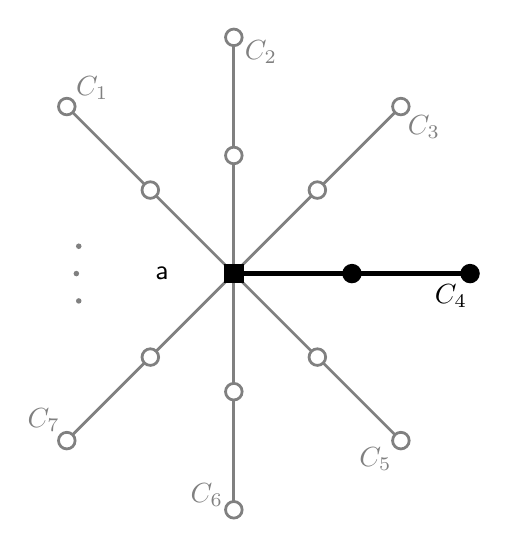
\begin{tikzpicture}
\tikzstyle{every path}=[line width=1pt]
\tikzstyle{every node}=[draw,line width=1pt,inner sep=0]

\tikzstyle{c1}=[rectangle,minimum size=6]

\tikzstyle{d1}=[circle,draw=none,fill,minimum size=2]

\tikzstyle{l7}=[draw=none,circle,minimum size=45]

\draw[gray] (0:0) -- (135:3)
	coordinate[c1,at start] (0)
	coordinate[c1,circle,midway,fill=white] (1)
	coordinate[c1,circle,at end,fill=white,label=35:$C_1$] (2);

\draw[gray] (0.center) -- (90:3)
	coordinate[c1,at start] (0)
	coordinate[c1,circle,midway,fill=white] (3)
	coordinate[c1,circle,at end,fill=white,label=350:$C_2$] (4);

\draw[gray] (0.center) -- (45:3)
	coordinate[c1,at start] (0)
	coordinate[c1,circle,midway,fill=white] (5)
	coordinate[c1,circle,at end,fill=white,label=305:$C_3$] (6);

\draw[gray] (0.center) -- (315:3)
	coordinate[c1,at start] (0)
	coordinate[c1,circle,midway,fill=white] (9)
	coordinate[c1,circle,at end,fill=white,label=215:$C_5$] (10);

\draw[gray] (0.center) -- (270:3)
	coordinate[c1,at start] (0)
	coordinate[c1,circle,midway,fill=white] (11)
	coordinate[c1,circle,at end,fill=white,label=170:$C_6$] (12);

\draw[gray] (0.center) -- (225:3)
	coordinate[c1,at start] (0)
	coordinate[c1,circle,midway,fill=white] (13)
	coordinate[c1,circle,at end,fill=white,label=125:$C_7$] (14);

\draw[black,line width=2pt] (0.center) -- (0:3)
	coordinate[c1,fill,at start] (0)
	coordinate[c1,circle,fill,midway] (7)
	coordinate[c1,circle,fill,at end,label=260:$C_4$] (8);

\coordinate[l7,label=180:${\textsf a}$] (0) at (0.center);

\coordinate[d1,gray] (.) at (190:2);
\coordinate[d1,gray] (.) at (180:2);
\coordinate[d1,gray] (.) at (170:2);
\end{tikzpicture}
\end{center}
\caption{
Greechie orthogonality diagram of a star-shaped configuration,
representing a common basis element/projector ${\textsf a}$ with an overlaid two-valued assignment reflecting $v({\textsf a})=1$.
Compare also Abbot, Calude, Conder \& K.S., eprint arXiv:1207.2029
}
\label{2012-psiqm-v2-f2}
\end{figure}

}

\frame{
\frametitle{Specker's ``bug'' diagram of ``phantom'' contexts}

\begin{figure}[h]
\begin{center}
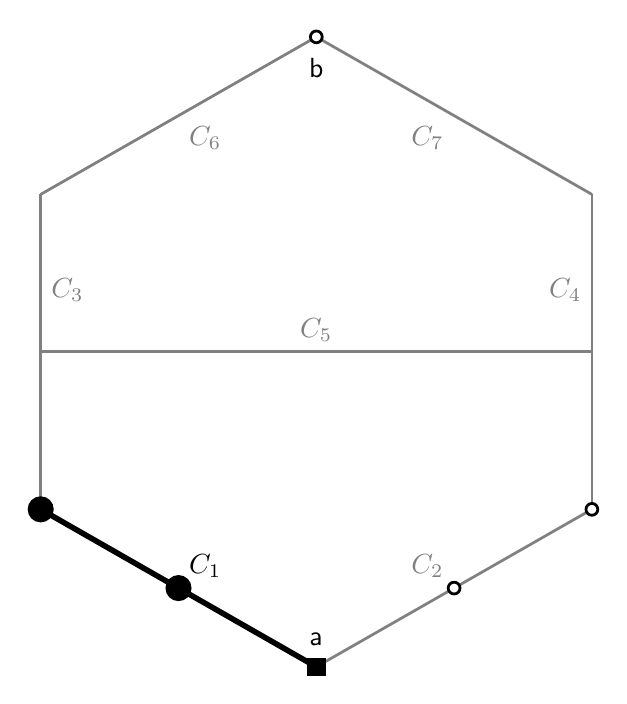
\begin{tikzpicture} [scale=0.5]

\tikzstyle{every path}=[line width=1pt]
\tikzstyle{c1}=[rectangle,minimum size=6]

%\draw[help lines,orange] (-7,-8) grid (7,8);


\draw[gray]  (7,4) -- (7,-4);
\node [above left, gray] at (7,1) {$C_4$};

\draw[gray]  (7,-4) -- (0,-8) ;
\node [above left, gray] at (3.5,-6) {$C_2$};
\draw[fill=white] (7,-4) circle [gray,radius=0.15];
\draw[fill=white] (3.5,-6) circle [gray,radius=0.15];

\draw[gray]  (-7,-4) -- (-7,4);
\node [above right, gray] at (-7,1) {$C_3$};

\draw[gray]  (-7,4) -- (0,8) ;
\node [below right, gray] at (-3.5,6) {$C_6$};

\draw[gray]  (0,8) -- (7,4);
\draw[fill=white] (0,8) circle [gray,radius=0.15];
\node [label=below:${\textsf b}$, gray] at (0,8) {};
\node [below left, gray] at (3.5,6) {$C_7$};


\draw[gray]  (-7,0) -- (7,0);
\node [above, gray] at (0,0) {$C_5$};

\draw [line width=2pt,black]  (0,-8) -- (-7,-4)
	coordinate[c1,circle, at end,fill=black] (0)
	coordinate[c1,circle,midway,fill=black] (1)
	coordinate[c1,rectangle,at start,fill=black] (2);
\node [above right, black] at (-3.5,-6) {$C_1$};
\node [label=above:${\textsf a}$, black] at (0,-8) {};

\end{tikzpicture}
\end{center}
\caption{
``Bug-type''  Greechie orthogonality diagram
with an overlaid two-valued assignment reflecting ``$v({\textsf a})=1$ implies $v({\textsf b})=0$.''
This configuration is part of the original
proof of the Kochen-Specker theorem.
For concrete coordinatizations, see, for instance, the original paper by Kochen and Specker, as well as Ref.~\cite{svozil-tkadlec,2012-incomput-proofsCJ}.
It is assumed that the system is prepared in state $C_1$, depicted by a block colored in thick filled black;
all the other sic contexts $C_2$--$C_7$ are   ``phantom contexts'' colored in gray.
}
\label{2012-psiqm-v2-f2}
\end{figure}

}


\frame{
\frametitle{Is the best interpretation of the quantum formalism its non-interpretation?}

Since around 1920 we are confronted with a situation in which an orthodoxy tries to supress and avoid thinking about the ``how'' -- c.f. Feynman's (in-)famous
dictum that while {\color{blue}``$\ldots$ nobody
understands quantum mechanics,''} to better stop thinking about these issues {\color{blue}``$\ldots$ if  you  can possibly avoid it.
because you will get
`down the drain', into a blind alley from which nobody has
yet escaped. Nobody knows how it can be like that.''});
or at least advises {\color{blue}``not worry too much''} (cf. Drac)
while at the same time expressing the opinion that certain events occur {\color{blue}{\it ex nihilo}} (out of nothing), fundamentally
inexplicably, and irreducibly random (cf. Zeilinger).

}

\frame{
\frametitle{Is the best interpretation of the quantum formalism its non-interpretation?-cntd.}

This, I believe, is tantamount to dogmatism,
and contradictory to all rationalistic principles on which scientific progress thrives.

I believe that there will be no significant scientific progress in this area without
attempts to give meaning to what is formalized.
Therefore, interpretation should not be discredited,
but considered wisely with {\em evenly-suspended attention}.

}


\section{Consequences for quantum random number generators}
\frame{
\frametitle{Consequences for quantum random number generators}

Where does the quantum randomness reside?

It is often taken for granted, that is miraculously emerges {\it ex nihilo} from those elements which perform in the Laplacian--unitary regime,
such as a beam splitters; but how can this happen?


I suggest to circumvent this conundrum is by postulating that
(i) at every instant, only a single state (or context) exists;
and that
(ii)
through {\em context translation,}
in which a mismatch between the preparation and the measurement results in the ``translation''
of the original information encoded by a quantum system into the answer requested,
noise is introduced by the many degrees of freedom of a suitable ``quasi-classical'' measurement apparatus.
This would be an altogether different source of randomness than irreducibly creation {\it ex nihilo} (``out of nothing'')
that is favoured by the present quantum orthodoxy.
}


\frame{

\centerline{\Large {\color{magenta} Thank you for your attention!}}

\begin{center}\color{orange}
$\widetilde{\qquad \qquad }$
$\widetilde{\qquad \qquad}$
$\widetilde{\qquad \qquad }$
\end{center}
 }
 \end{document}
